\documentclass[tikz,border=6pt]{standalone}
\usepackage{pgfplots}
\usepgfplotslibrary{groupplots}
\usetikzlibrary{calc}
\pgfplotsset{compat=1.18}
\begin{document}
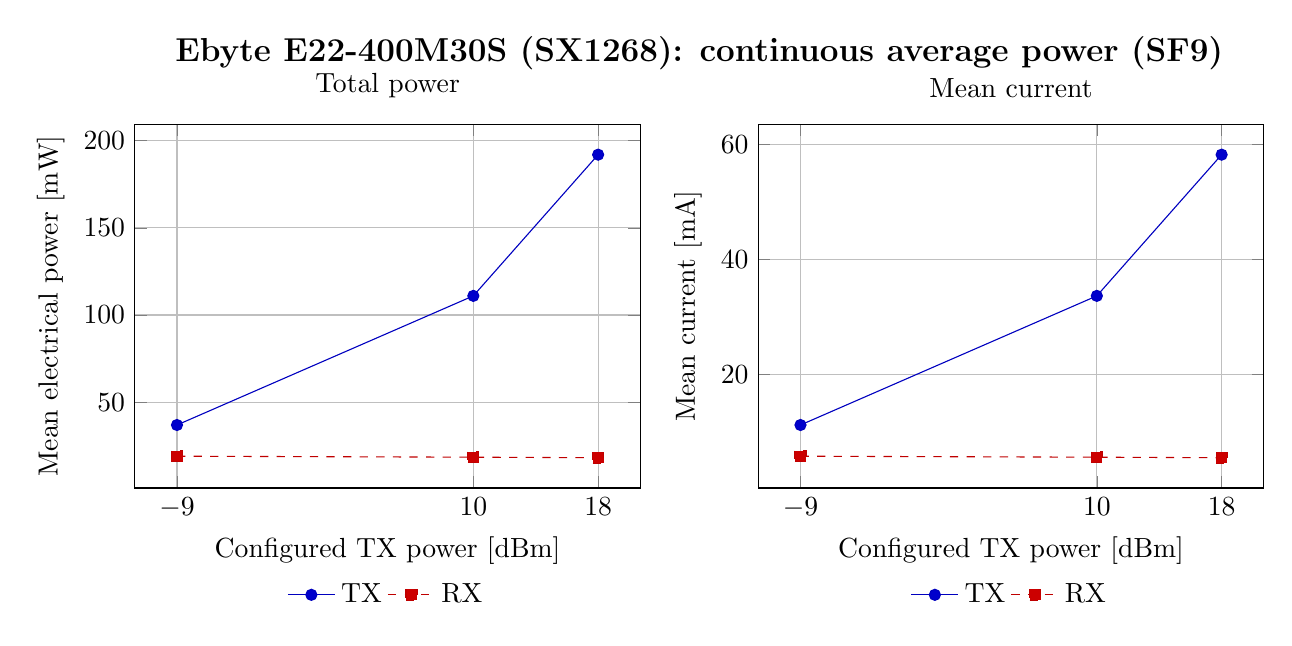
\begin{tikzpicture}
\begin{groupplot}[group style={group size=2 by 1,horizontal sep=1.5cm},width=8cm,height=6.2cm,xtick={-9,10,18},xlabel={Configured TX power [dBm]},grid=both,legend style={draw=none,at={(0.5,-0.23)},anchor=north,legend columns=2}]
\nextgroupplot[title={Total power},ylabel={Mean electrical power [mW]}]
\addplot+[blue!75!black,mark=*] coordinates {(-9,36.909358) (10,110.961215) (18,191.934327)};\addlegendentry{TX}
\addplot+[red!75!black,dashed,mark=square*] coordinates {(-9,19.0149169) (10,18.4494162) (18,18.1500015)};\addlegendentry{RX}
\nextgroupplot[title={Mean current},ylabel={Mean current [mA]}]
\addplot+[blue!75!black,mark=*] coordinates {(-9,11.1846539) (10,33.6246106) (18,58.1619172)};\addlegendentry{TX}
\addplot+[red!75!black,dashed,mark=square*] coordinates {(-9,5.76209604) (10,5.59073219) (18,5.50000045)};\addlegendentry{RX}
\end{groupplot}
\node[font=\bfseries\large] at ($(group c1r1.north)!0.5!(group c2r1.north)+(0,0.9cm)$) {Ebyte E22-400M30S (SX1268): continuous average power (SF9)};
\end{tikzpicture}
\end{document}
